% Add `ngerman` to documentclass for German docs
\documentclass[12pt, a4paper]{article}
\usepackage{a4wide}
\usepackage{setspace}
\usepackage{csquotes}
\usepackage[utf8]{inputenc}

\usepackage{url}
\usepackage[hidelinks]{hyperref}
\usepackage{minted}
\usemintedstyle{perldoc}

% inline code
\newcommand{\code}[1]{\texttt{#1}}

% Uncomment for German
%\usepackage[ngerman]{babel}

% For generating template dummy text
\usepackage{lipsum}

\usepackage{myColors}
\usepackage{myFooter}
\usepackage{myTitle}

% Libraries outside of template
\usepackage[T1]{fontenc}
\usepackage{upquote}
\AtBeginDocument{%
    \def\PYZsq{\textquotesingle}%
}

\usepackage{amsmath}

\usepackage{verbatim}

\usepackage{longtable}

\usepackage{adjustbox}

%%%%%%%%%%%%%%%%%%%%%%%%%%%%%%%%%%%%%%%%%%%%%%%%%%%%%%%%%%%%%%%%%%%%%%%%%%%%%%%%

\project{CS 432 Web Science}
\author{Derek Goddeau}
\title{Assignment Ten}
\supervisor{Michael L. Nelson}

\doublespace
\pagestyle{hacker}

\begin{document}
\maketitle

\newpage



%%%%%%%%%%%%%%%%%%%%%%%%%%%
% Get classificaiton data %
%%%%%%%%%%%%%%%%%%%%%%%%%%%
\section{Use knnestimate() to compute nearest neighbors}
 
For this I worked from the interactive prompt after only slight modifications to the PCI code it was just the following commands to generate the tables.

\begin{minipage}{\linewidth} % prevent splitting between pages
\vspace{2em}
\begin{minted}[fontfamily=tt]{python}
>>> import clusters
>>> import numpredict
>>> from tabulate import tabulate
>>> from collections import OrderedDict
>>> blognames, words, data = clusters.readfile(filename)
>>> f_measure_table = OrderedDict()
>>> for k in [1, 2, 5, 10, 20]:
...     numpredict.knnestimate(data, data[blognames.index('F-Measure')], k=k)
...
>>> tabulate(f_measure_table, headers='keys', tablefmt='latex')
\end{minted}
\vspace{2em}
\end{minipage}

\begin{table}[ht]
\centering
\caption{http://f-measure.blogspot.com/}
\begin{adjustbox}{width=1\textwidth}
\small
\begin{tabular}{lllll}
\hline
 k = 1         & k = 2           & k = 5                & k = 10               & k = 20                                        \\
\hline
 Laganas rock! & Laganas rock!   & Laganas rock!        & Laganas rock!        & Laganas rock!                                 \\
               & Banging Windows & Banging Windows      & Banging Windows      & Banging Windows                               \\
               &                 & The Travels of Dave  & The Travels of Dave  & The Travels of Dave                           \\
               &                 & Design Your World    & Design Your World    & Design Your World                             \\
               &                 & Myths.. MyThoughts.. & Myths.. MyThoughts.. & Myths.. MyThoughts..                          \\
               &                 &                      & The Wizard and I.    & The Wizard and I.                             \\
               &                 &                      & Girl Informer        & Girl Informer                                 \\
               &                 &                      & SOPHIE PATTERSON     & SOPHIE PATTERSON                              \\
               &                 &                      & RED PAPER ONLINE     & RED PAPER ONLINE                              \\
               &                 &                      & Kaleidoscope         & Kaleidoscope                                  \\
               &                 &                      &                      & Star's Adventures at Camp Half Blood          \\
               &                 &                      &                      & Dream, sports, and Travel Blogs               \\
               &                 &                      &                      & What's in my head...                          \\
               &                 &                      &                      & The Fat Lady                                  \\
               &                 &                      &                      & The Original Runaway Heart                    \\
               &                 &                      &                      & Brent and Paulette's Excellent RV Adventure's \\
               &                 &                      &                      & Serendipity                                   \\
               &                 &                      &                      & The Pink Lady of Hollywood                    \\
               &                 &                      &                      & poetic illusions                              \\
               &                 &                      &                      & All Feet are the Same!                        \\
\hline
\end{tabular}
\end{adjustbox}
\end{table}

\newpage
\noindent
The results seem alright for F-Measure but I am not so sure about for the Web Science blog.

\begin{table}[ht]
\centering
\caption{http://ws-dl.blogspot.com/}
\begin{adjustbox}{width=1\textwidth}
\small
\begin{tabular}{lllll}
\hline
 k = 1         & k = 2             & k = 5             & k = 10               & k = 20                         \\
\hline
 Girl Informer & Girl Informer     & Girl Informer     & Girl Informer        & Girl Informer                  \\
               & Design Your World & Design Your World & Design Your World    & Design Your World              \\
               &                   & The Wizard and I. & The Wizard and I.    & The Wizard and I.              \\
               &                   & mayur             & mayur                & mayur                          \\
               &                   & RED PAPER ONLINE  & RED PAPER ONLINE     & RED PAPER ONLINE               \\
               &                   &                   & Kaleidoscope         & Kaleidoscope                   \\
               &                   &                   & Random Thoughts      & Random Thoughts                \\
               &                   &                   & Myths.. MyThoughts.. & Myths.. MyThoughts..           \\
               &                   &                   & SOPHIE PATTERSON     & SOPHIE PATTERSON               \\
               &                   &                   & The Fat Lady         & The Fat Lady                   \\
               &                   &                   &                      & poetic illusions               \\
               &                   &                   &                      & The Travels of Dave            \\
               &                   &                   &                      & Rhiannon's A2 Media Coursework \\
               &                   &                   &                      & Banging Windows                \\
               &                   &                   &                      & NOSTALGIA                      \\
               &                   &                   &                      & What's in my head...           \\
               &                   &                   &                      & the silhouette of a dream.     \\
               &                   &                   &                      & Babe in Old Town               \\
               &                   &                   &                      & Damon @ Awahono School         \\
               &                   &                   &                      & The Original Runaway Heart     \\
\hline
\end{tabular}
\end{adjustbox}
\end{table}


\newpage
\section{Rerun A9, Q2 using LIBSVM}

I again made use of the \href{https://github.com/hylang/hy}{hy} code for dictionary manipulations. I used \href{http://scikit-learn.org/stable/documentation.html}{scikit-learn} packages \href{http://scikit-learn.org/stable/modules/svm.html}{SVM library} to access the Python LIBSVM bindings. From it I used the \href{http://scikit-learn.org/stable/modules/generated/sklearn.svm.SVC.html#sklearn.svm.SVC}{SVC} classifier since it supports multi-class classification in a "one-against-one" approach and \code{LinearSVC} uses a one against the rest method.

This approach required more massaging of the data to get it into a form that \code{SVC} wanted, and that could also show the requested data but it greatly simplified it overall. Since \code{SVC} wants parallel vectors as input, both numeric I used the \href{http://scikit-learn.org/stable/modules/generated/sklearn.preprocessing.LabelEncoder.html}{sklearn.preprocessing.LableEncoder} to translate the labels back and forth and the preprocessing \href{http://scikit-learn.org/stable/modules/preprocessing.html#preprocessing}{data standardization} functions to normalize the data.

In all the program is not really much different, it follows the same pattern. For cross validation I split the dictionary using into a larger dictionary containing all of the needed training and testing pairs and pass each to the classifier. I had to visit the parentheses mine they hide behind MIT for the \code{hy} code on this one though. From each result I generate and save a confusion matrix class like for assignment nine. The heatmap of a single run is shown in figure~\ref{fig:svm} on page~\pageref{fig:svm}.

\begin{table}[H]
    \centering
    \caption{Accuracy}
    \label{tab:5050}
    \begin{tabular}{lc}
    \hline
    Category    & Percent Correct \\
    \hline
    admin       & 68\%  \\
    commands    & 45\%  \\
    off-topic   & 73\%  \\
    plugins     & 84\%  \\
    vimrc       & 80\%  \\
    mappings    & 85\%  \\
    \hline
    \end{tabular}
\end{table}

\begin{figure}[H]
    \label{fig:svm}
    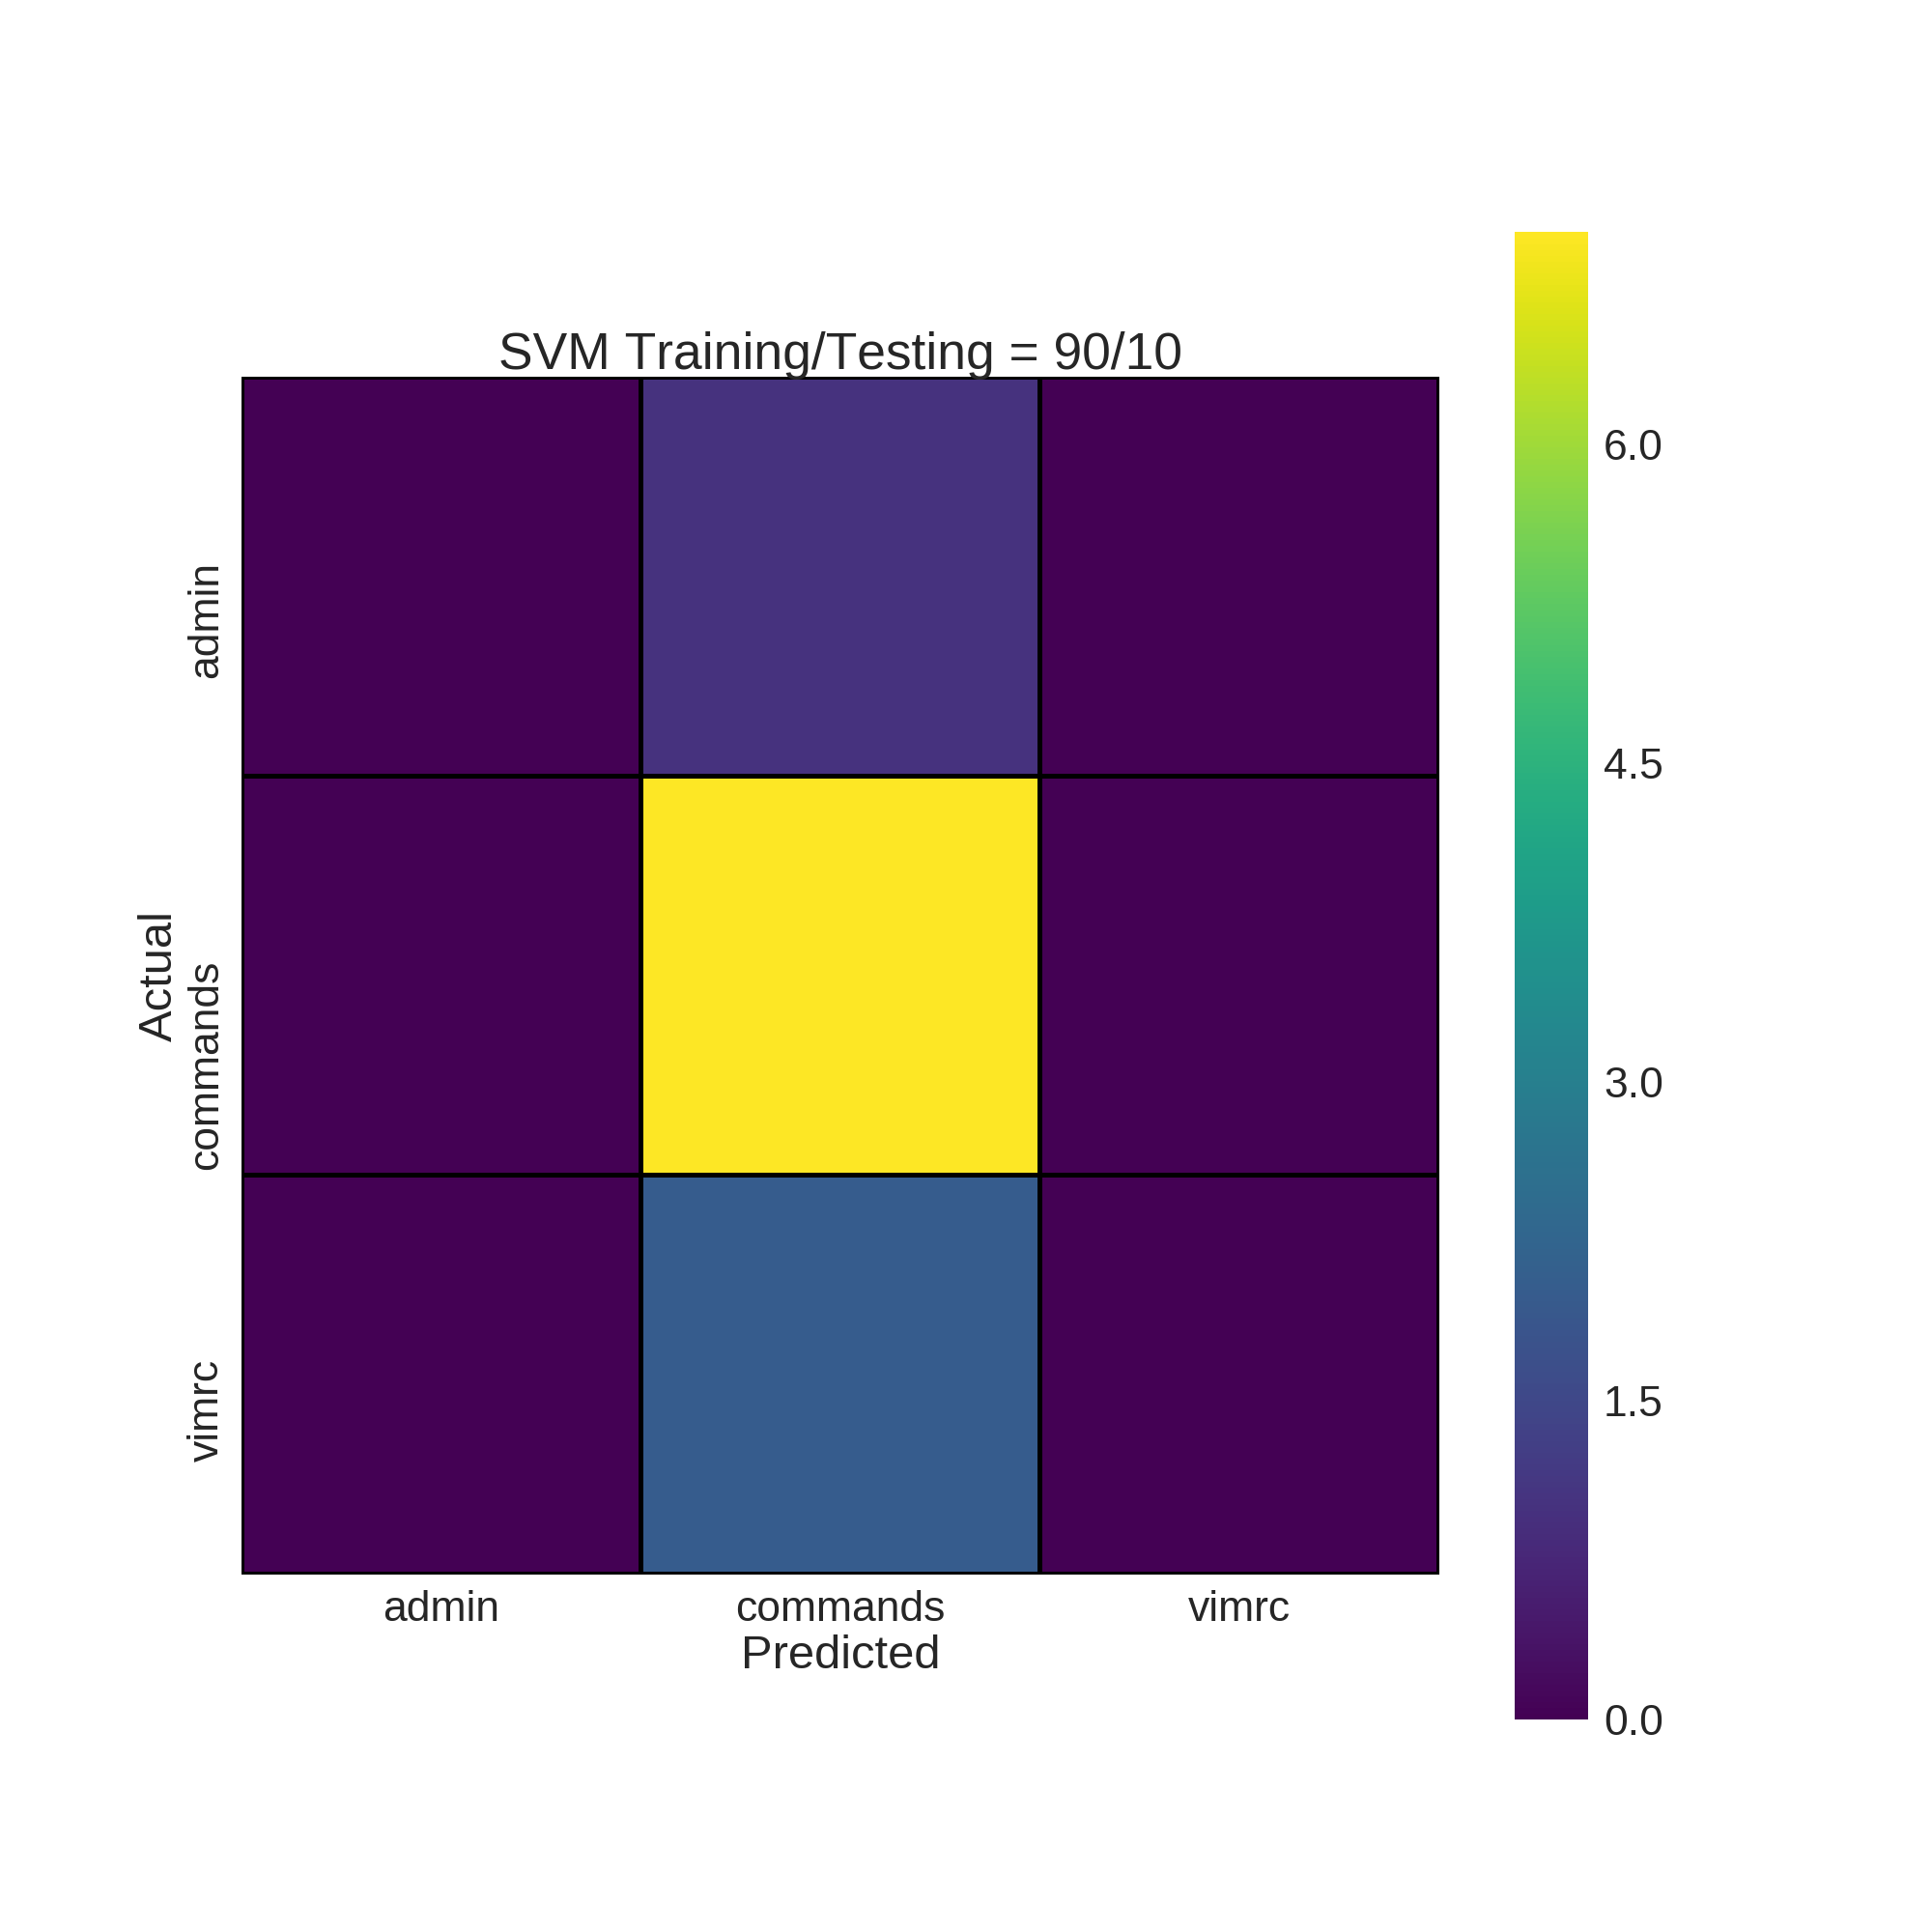
\includegraphics[width=\textwidth]{../train_validate_libsvm/heatmaps/svm.png}
\end{figure}

\begin{minipage}{\linewidth} % prevent splitting between pages
\vspace{2em}
\begin{minted}[fontfamily=tt]{clojure}
(defn remove-keys [dictionary keys &optional [inverse None]]
  "Remove given keys from a dictionary"
  (if-not inverse
    (dict-comp k (get dictionary k) [k (.keys dictionary)] (not-in k keys))
    (dict-comp k (get dictionary k) [k (.keys dictionary)] (in k keys))))

(defn chunks [dictionary percentage]
  "Split dictionary into even dictionary chunks"
  (setv chunk-size (int (* (len dictionary) percentage)))
  (setv i (iter (.keys dictionary)))
  (for (xs (range 0 (len (.keys dictionary)) chunk-size))
    (yield (dict-comp k (get dictionary k) [k (islice i chunk-size)]))))

(defn k-fold [dictionary &optional [k 0.1]]
  "Given a dictionary return a list of the k-fold dictionaries"
  (setv acc [])
  (for (chunk (chunks dictionary k))
    (.append acc chunk)) acc)

(defn k-combinations [dictionary &optional [k 0.1]]
  "Get k-fold of dictionary then create list of all possible combinations"
  (setv acc [])
  (for (fold (k-fold dictionary :k k))
    (.append acc
      {"validation" fold "training" (remove-keys dictionary (.keys fold))})) acc)
\end{minted}
\vspace{2em}
\end{minipage}

\end{document}
